\documentclass[12pt]{article}
\usepackage[margin=1in]{geometry}
\usepackage{amsmath}
\usepackage{booktabs}
\usepackage{graphicx}
\usepackage{tikz}
\usepackage{mathtools}  
\usepackage{xfrac}  
\usepackage[section]{placeins}
\usetikzlibrary{automata,positioning,arrows}
\newcommand\tab[1][1cm]{\hspace*{#1}} \newcommand\n{\newline}
\newcommand\partiald[2]{
    \frac{\partial #1}{\partial #2}
} \newcommand\ra{\rightarrow}

\begin{document}
CS7347 Test 2, Noah Gardner, 000843905\n

% P1
\section*{Question 1}
\textbf{[Points 15]} A grammar is ambiguous if it can generate a string two or
more ways. In other words, a string generated by the grammar does not have a
unique parse tree.

Given grammar:

\begin{tabular}{lll}
      S & $\rightarrow$ & a B $|$ b A         \\
      A & $\rightarrow$ & a $|$ a S $|$ b A A \\
      B & $\rightarrow$ & b $|$ b S $|$ a B B \\
\end{tabular}

Is the above grammar ambiguous? Provide an example and show parse tree to
validate your answer.

\textbf{Answer:} The grammar is ambiguous because there exists two distinct
parse trees for the string \verb/aababbb/. The two parse trees are shown below:

\begin{figure}[!ht]
      \centering
      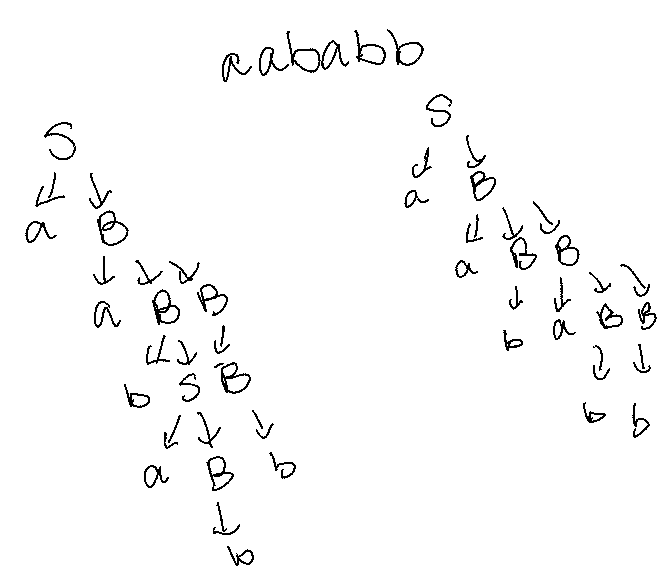
\includegraphics[width=0.6\textwidth]{assets/test2/p1.png}
\end{figure}


% P2
\newpage
\section*{Question 2}
\textbf{[Points 15]} Describe issue of BLEU Score. Given candidate translation
sentences and their references below, compute modified BLEU score.

\noindent\textbf{Candidate 1:} It is a guide to action which ensures that the military
always obeys the commands of the party.

\noindent\textbf{Candidate 2:} It is to ensure the troops forever hearing the activity
guidebook that party direct.

\noindent\textbf{Reference 1:} It is a guide to action that ensures that the military
will forever heed Party commands.

\noindent\textbf{Reference 2:} It is the guiding principle which guarantees the military
forces always being under the command of the Party.

\noindent\textbf{Reference 3:} It is the practical guide for the army always to heed the
directions of the party.

Evaluate your translation model performance using BLEU score where $n$-gram
order, $N=2$. Please show the best reference during your computation.

\textbf{Answer:} The BLEU score is computed using the modified formula, where
the geometric mean of each $n$-gram precision is computed.
\begin{table}[!ht]
      \centering
      \begin{tabular}{|rll|l|}
            \hline
            Candidate & Unigram & Bigram & Modified BLEU \\
            \hline
            $1$       & $0.95$  & $0.61$ & $0.76$        \\
            $2$       & $0.53$  & $0.06$ & $0.18$        \\
            \hline
      \end{tabular}
\end{table}

The best reference for the modified BLEU score is reference $1$, as shown in the
table below.

\begin{table}[!ht]
      \centering
      \begin{tabular}{|r|rll|l|}
            \hline
            Reference & Candidate & Unigram & Bigram & Modified BLEU \\
            \hline
            $1$       & $1$       & $0.63$  & $0.44$ & \textbf{0.53} \\
                      & $2$       & $0.41$  & $0.06$ & \textbf{0.16} \\
            \hline
            $2$       & $1$       & $0.53$  & $0.17$ & $0.30$        \\
                      & $2$       & $0.26$  & $0.05$ & $0.12$        \\
            \hline
            $3$       & $1$       & $0.58$  & $0.22$ & $0.36$        \\
                      & $2$       & $0.41$  & $0.06$ & $0.16$        \\
            \hline
      \end{tabular}
\end{table}

% P3
\newpage
\section*{Question 3}
\textbf{[Points 10]} Given a grammar below

\begin{tabular}{lll}
      \hline
      NP  & $\rightarrow$ & Det $|$ Nom                            \\
      Nom & $\rightarrow$ & AP $|$ Nom                             \\
      AP  & $\rightarrow$ & Adv $|$ A                              \\
      \hline
      Det & $\rightarrow$ & a $|$ an                               \\
      Adv & $\rightarrow$ & very $|$ extremely                     \\
      AP  & $\rightarrow$ & heavy $|$ orange $|$ tall              \\
      A   & $\rightarrow$ & heavy $|$ orange $|$ tall $|$ muscular \\
      Nom & $\rightarrow$ & book $|$ orange $|$ man                \\
      \hline
\end{tabular}

Show a parse tree for the following sentences:

\textbf{Sentence 1:} A very heavy orange book

\textbf{Sentence 2:} A very tall extremely muscular man

\textbf{Answer:}

\begin{figure}[!ht]
      \centering
      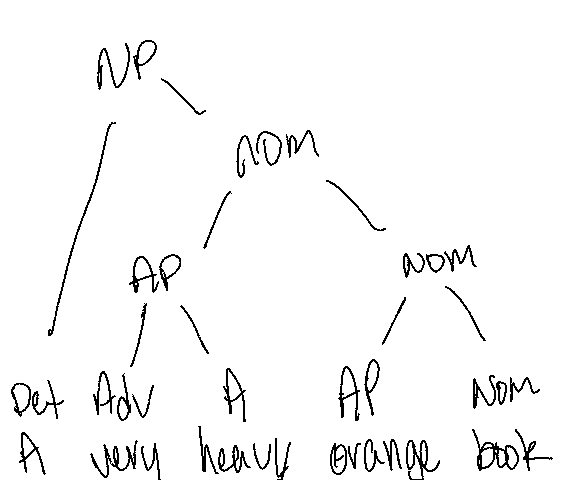
\includegraphics[width=0.55\textwidth]{assets/test2/p3a.png}
\end{figure}

\begin{figure}[!ht]
      \centering
      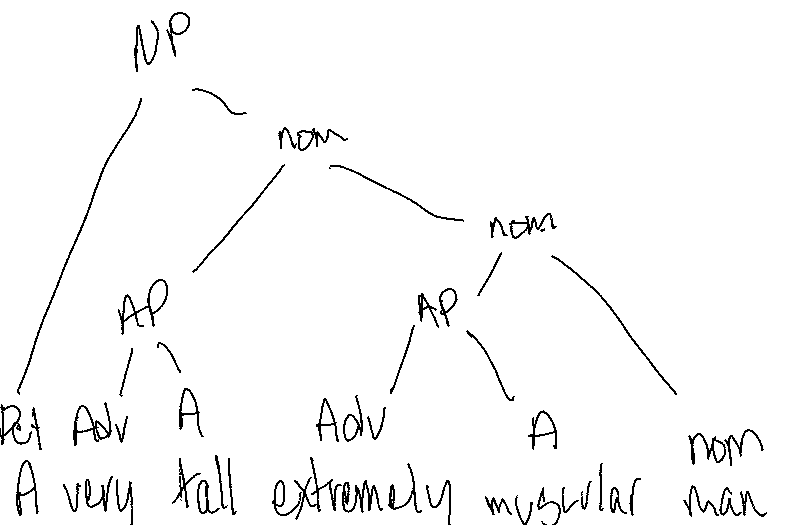
\includegraphics[width=0.55\textwidth]{assets/test2/p3b.png}
\end{figure}

% P4
\newpage
\section*{Question 4}
\textbf{[Points 5]} Write down the differences between attachment ambiguity and
coordination ambiguity.

\textbf{Answer:} Attachment ambiguity occurs when it is uncertain where a phrase
or clause should be attached to a sentence. In the example: "I saw the man with
the telescope.", the prepositional phrase can be attached as a noun phrase or a
verb phrase. In otherwords, it's unclear whether "I saw the man holding the
telescope." or "I saw the man through the telescope."

Coordination ambiguity occurs when different phrases can be coinjoined with
conjunctions such as "and" or "or". For example, in a sentence that can modify
both sides of the conjunction as in "secure hardware and software", it is
ambiguous if both the hardware and software are secure, or if only the hardware
is secure.

% P5
\newpage
\section*{Question 5}
\textbf{[Points 15]} Suppose you build two summarizer systems, and your systems
generates the following summary. You named your summarizer as S1 and S2,
respectively. You are also given reference summary below.

\textbf{S1 Summary:} neymar scored his side's second goal with a curling free
kick, and 15 minutes to play in the 2-2 draw at sevilla on saturday night,
according to reports in spain.

\textbf{S2 Summary:} barcelona's neymar substituted in 2-2 draw at sevilla on
saturday night, spain's kamui kobayashi claims a late free kick in the champions
league after his second goal with the score

\textbf{Reference summary:} neymar was taken off with barcelona 2-1 up against
sevilla. the brazil captain was visibly angry, and barca went on to draw 2-2.
neymar has been replaced 15 times in 34 games this season. click here for all
the latest barcelona news.

Please compute the performance of your system using ROUGE-1 and ROUGE-2 -
precision, recall, and f1 score metrics and compare both systems with respective
ROUGE metrics (e.g., ROUGE-1 S1 vs. ROUGE-1 S2). Based on your comparison, which
one of the ROUGE metrics would you select to evaluate your system performance?

\textbf{Answer:} I would choose the F1 metric, since it contains information
from both precision and recall. My scores are calculated after removing
punctuation and tokenizing each summary.

\begin{table}[!ht]
      \centering
      \begin{tabular}{|r|lll|}
            \hline
            System     & Precision & Recall & F1   \\
            \hline
            ROUGE-1 S1 & 0.34      & 0.25   & 0.29 \\
            ROUGE-1 S2 & 0.27      & 0.20   & 0.23 \\
            \hline
            ROUGE-2 S1 & 0.03      & 0.02   & 0.03 \\
            ROUGE-2 S2 & 0.03      & 0.02   & 0.03 \\
            \hline
      \end{tabular}
\end{table}
% P6
\newpage
\section*{Question 6}
\textbf{[Points 5]} Given a grammar below

\begin{tabular}{|lll|}
      \hline
      S  & $\rightarrow$ & NP VP \\
      \hline
      VP & $\rightarrow$ & Vi    \\
      VP & $\rightarrow$ & Vt NP \\
      VP & $\rightarrow$ & VP PP \\
      \hline
      NP & $\rightarrow$ & DT NN \\
      NP & $\rightarrow$ & NP PP \\
      \hline
      PP & $\rightarrow$ & IN NP \\
      \hline
\end{tabular}

\begin{tabular}{|lll|}
      \hline
      Vi & $\rightarrow$ & 'sleeps'    \\
      Vt & $\rightarrow$ & 'saw'       \\
      \hline
      NN & $\rightarrow$ & 'man'       \\
      NN & $\rightarrow$ & 'woman'     \\
      NN & $\rightarrow$ & 'telescope' \\
      NN & $\rightarrow$ & 'dog'       \\
      \hline
      DT & $\rightarrow$ & 'the'       \\
      \hline
      IN & $\rightarrow$ & 'with'      \\
      IN & $\rightarrow$ & 'in'        \\
      \hline
\end{tabular}

Show that this grammar is ambiguous and produces two different parse tree for
the following sentence.

\textbf{Sentence:} the man saw the dog with the telescope

\textbf{Answer:}

\begin{figure}[!ht]
      \centering
      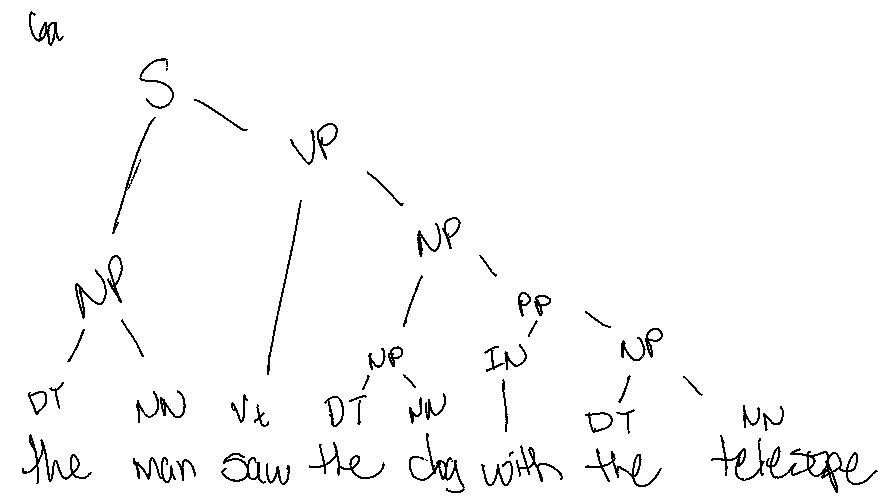
\includegraphics[width=0.5\textwidth]{assets/test2/p6a.png}
\end{figure}

\begin{figure}[!ht]
      \centering
      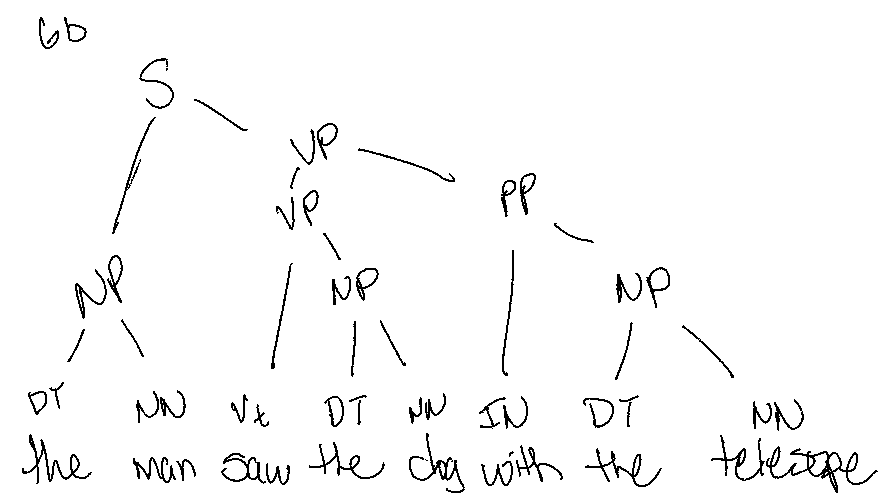
\includegraphics[width=0.5\textwidth]{assets/test2/p6b.png}
\end{figure}

% P7
\newpage
\section*{Question 7}
\textbf{[Points 20]} Evaluate the following example and compute precision,
recall and F1 scores.

\begin{figure}[!ht]
      \centering
      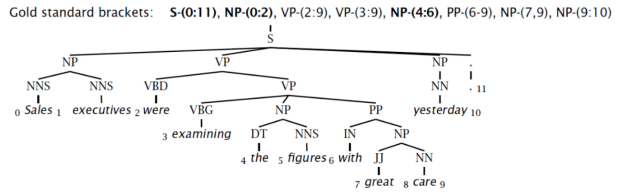
\includegraphics[width=0.95\textwidth]{assets/test2/gold_standard_brackets.png}
\end{figure}

\begin{figure}[!ht]
      \centering
      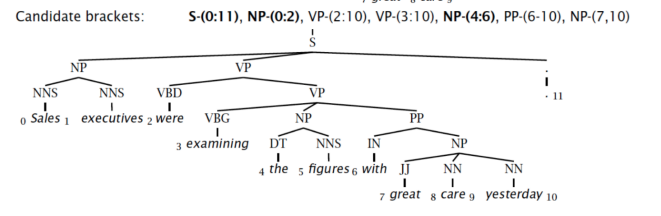
\includegraphics[width=0.95\textwidth]{assets/test2/candidate_brackets.png}
\end{figure}

\textbf{Answer:} The only node in the wrong position is node (yesterday, 10).
The metrics are listed in the table below.

\begin{table}[ht]
      \centering
      \begin{tabular}{rl}
            \hline
            Correct Nodes       & 10   \\
            Candidate Nodes     & 11   \\
            Gold Standard Nodes & 11   \\
            \hline
            Precision           & 0.91 \\
            Recall              & 0.91 \\
            F1                  & 0.91 \\
            \hline
      \end{tabular}
\end{table}


% P8
\newpage
\section*{Question 8}
\textbf{[Points 5]} In transition-based parsing we see dependency structure were
provided, then why we need to parse the sentence while given the structures?

\textbf{Answer:} Although the dependency structure is provided, we must perform
transition-based parsing in order to find a derivation for the input sentence.
In other words, we seek the configuration where the sentence can be represented
as a dependency tree. If we can't form a derivation for the sentence, that means
the sentence can not be interpreted with the provided dependency structure, and
if this result is unexpected, we should reevaulate either the dependency
structure or the sentence.

% P9
\newpage
\section*{Question 9}
\textbf{[Points 5]} What is CNF form? Why is Chomsky Normal Form used?

\begin{tabular}{lll}
      S & $\rightarrow$ & a X b X              \\
      X & $\rightarrow$ & a Y $|$ b Y $|$ null \\
      Y & $\rightarrow$ & X $|$ c              \\
\end{tabular}


Convert this CFG to CNF.

\textbf{Answer:} Chomsky Normal Form (CNF) is a method of representation for a
context-free grammar. Generating rules in CNF follow one of the following rules:

\begin{itemize}
      \item Rule must expand to two non-terminals.
      \item Rule must expand to exactly one terminal.
\end{itemize}

By adhering to CNF, we can use the Cocke-Kasami-Younger (CKY) algorithm to
easily parse strings and see if they are in the language of the context-free
grammar.

\begin{figure}[!ht]
      \centering
      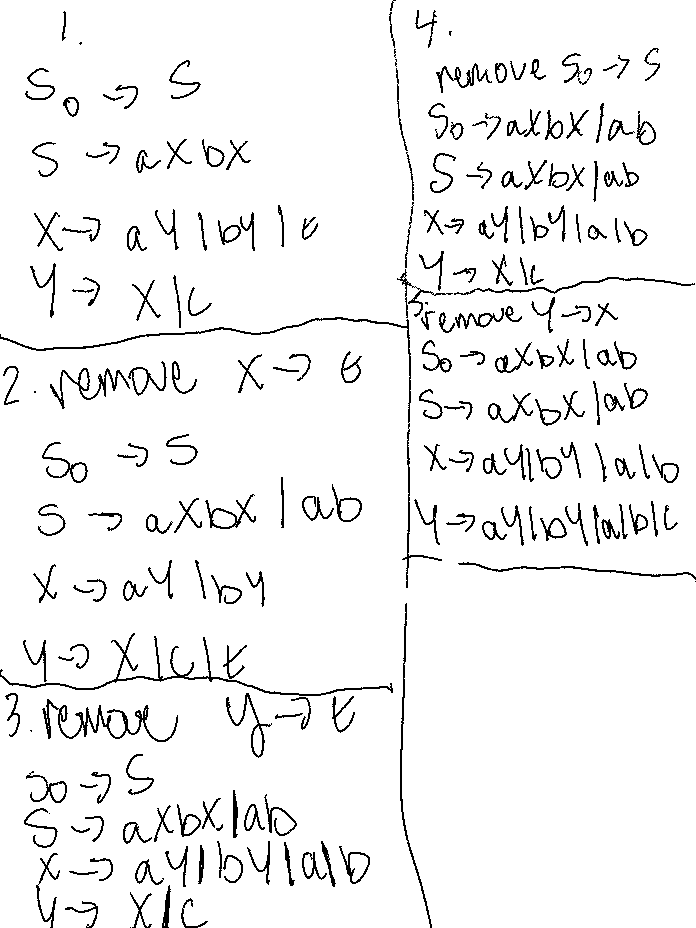
\includegraphics[width=0.6\textwidth]{assets/test2/p9a.png}
\end{figure}
\newpage

\begin{figure}[!ht]
      \centering
      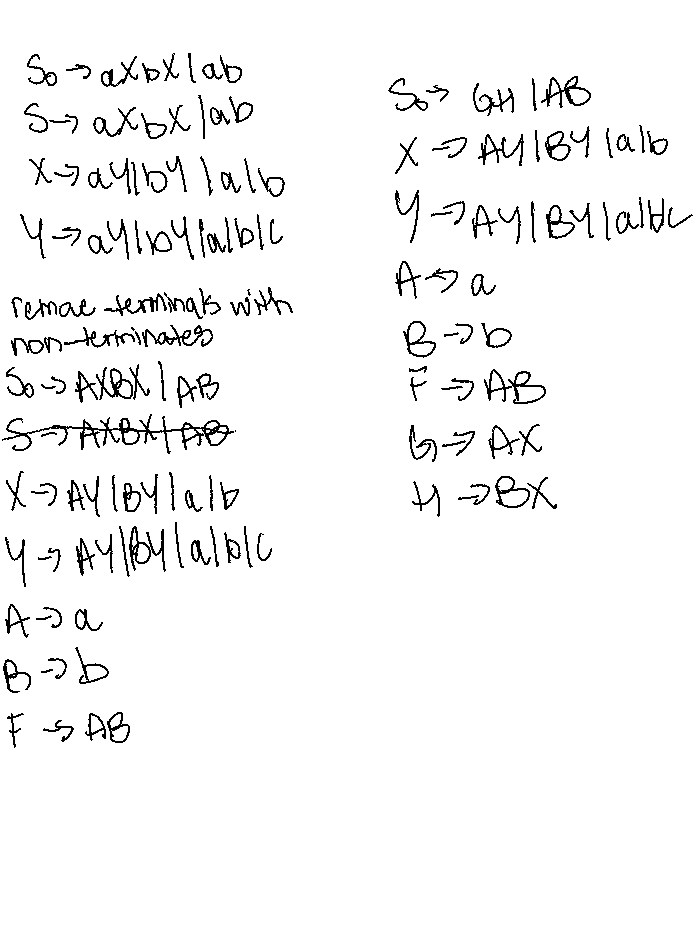
\includegraphics[width=0.6\textwidth]{assets/test2/p9b.png}
\end{figure}

Final CNF grammar:
\begin{table}[!ht]
      \begin{tabular}{lll}
            $S_0$ & $\rightarrow$ & GH $|$ AB                   \\
            X     & $\rightarrow$ & AY $|$ BY $|$ a $|$ b       \\
            Y     & $\rightarrow$ & AY $|$ BY $|$ a $|$ b $|$ c \\
            A     & $\rightarrow$ & a                           \\
            B     & $\rightarrow$ & b                           \\
            G     & $\rightarrow$ & AX                          \\
            H     & $\rightarrow$ & BX                          \\
      \end{tabular}
\end{table}

% P10
\newpage
\section*{Question 10}
\textbf{[Points 5]} How would you encode sentence using deep neural network?
Show details architecture of your network with an example sentence.

A recurrent neural network (RNN) may be used to encode a sentence. An RNN is
similar to a feedforward network, but instead of a single linear layer, it has a
hidden layer of recurrent units, which allows it to receive time-dependent
inputs, such as how words in a sentence depend on the previous word. We can keep
the output layer of the RNN as a fixed vector, and use it as a fixed feature
vector for the sentence. In this way, we can use the RNN to encode sentences
without having to learn a separate word embedding. If we wish, we may also use a
decoder model in order to train our encoder. An example architecture for the
encoder is shown below. For simplicity, there are only 2 hidden layers shown,
but a neural network is considered deep when it has many hidden layers.

\begin{figure}
      \centering
      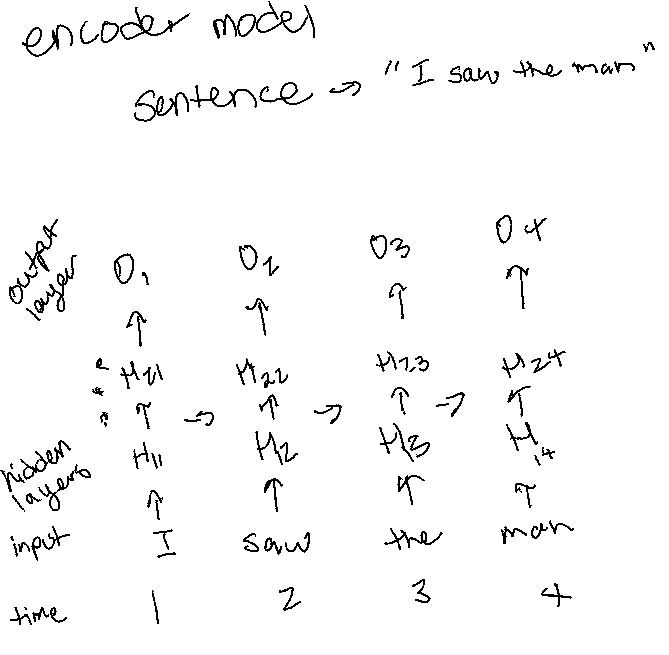
\includegraphics[width=0.8\textwidth]{assets/test2/p10.png}
\end{figure}
\end{document}